%% LyX 2.1.3 created this file.  For more info, see http://www.lyx.org/.
%% Do not edit unless you really know what you are doing.
\documentclass[english]{exam}
\usepackage[T1]{fontenc}
\usepackage[latin1]{inputenc}
\usepackage{float}
\usepackage{amstext}
\usepackage{graphicx}
\usepackage{setspace}
\usepackage{units}
\onehalfspacing

\makeatletter
%%%%%%%%%%%%%%%%%%%%%%%%%%%%%% Textclass specific LaTeX commands.

            

%%%%%%%%%%%%%%%%%%%%%%%%%%%%%% User specified LaTeX commands.
%% LyX 1.4.2 created this file.  For more info, see http://www.lyx.org/.
%% Do not edit unless you really know what you are doing.



\usepackage{float,calc,color}

\makeatletter

%%%%%%%%%%%%%%%%%%%%%%%%%%%%%% LyX specific LaTeX commands.
%% A simple dot to overcome graphicx limitations

%% Frontmatter vars
\def\thetitle#1{\gdef\@thetitle{#1}}
\def\thedate#1{\gdef\@thedate{#1}}




% ******************************************************************
% *** SPACE CONTROL ************************************************

\def\vf{\vfill}
\def\vs{\vspace{1pc}}
\def\hs{\hspace{1in}}

\def\blank{$\,$ \underline{\hspace{1in}} $\,$}
\def\Blank{$\,$ \underline{\hspace{1.5in}} $\,$}

\def\cpg{\clearpage}

% ******************************************************************
% *** FORMATTING ***************************************************

\def\und{\underline}

% ******************************************************************
% *** ENGLISH ABBREVIATIONS ****************************************

\def\ie{\mbox{{\it i.e.} }}
\def\eg{\mbox{{\it e.g.} }}
\def\etc{\mbox{{\it et cetera} }}

% ******************************************************************
% *** MATH SHORTCUTS ***********************************************

\def\ds{\displaystyle}

\def\ddx{\ds \frac{d}{dx}}
\def\ddt{\ds \frac{d}{dx}}
\newcommand{\dd}[2]{\ds \frac{d{#1}}{d{#2}}}

\def\pitch{\mathbin{\frown \! \! \! \! \mid \, \, \,}}  % replace by \pitchfork if amssymb is working

\def\qed{\rule[-.23ex]{1.6ex}{1.6ex}}

% ******************************************************************
% *** TABLE SHORTHAND **********************************************

\newcommand{\gotable}[3]
      {\begin{table}[h] 
       \begin{center}
       \addtolength{\tabcolsep}{#1mm}
       \renewcommand{\arraystretch}{#2}
       \begin{tabular}{#3}}

\newcommand{\stoptable}
      {\end{tabular}
       \end{center}
       \end{table}}
       
% ******************************************************************
% *** MINIPAGE SHORTHAND *******************************************

\newcommand{\twofig}[4]
   {\begin{figure}[h]
      \begin{minipage}[t]{3in}
        \begin{center}
        {\Large \bf (#1) $\!\!\!\!\!\!\!\!\!$}
        \epsfig{file=#2,height=2in,width=2in} 
        \end{center}
      \end{minipage}
      \hfill
      \begin{minipage}[t]{3in}
        \begin{center}
        {\Large \bf (#3) $\!\!\!\!\!\!\!\!\!$}
        \epsfig{file=#4,height=2in,width=2in}  
        \end{center}
      \end{minipage}
    \end{figure}}

\newcommand{\threefig}[6]
   {\begin{figure}[h]
      \begin{minipage}[t]{2in}
        \begin{center}
        {\large \bf (#1) $\!\!\!\!\!\!\!\!\!$}
        \epsfig{file=#2,height=1.6in,width=1.6in}
        \end{center}
      \end{minipage}
      \hfill
      \begin{minipage}[t]{2in}
        \begin{center}
        {\large \bf (#3) $\!\!\!\!\!\!\!\!\!$}
        \epsfig{file=#4,height=1.6in,width=1.6in}
        \end{center}
      \end{minipage}
      \hfill
      \begin{minipage}[t]{2in}
        \begin{center}
        {\large \bf (#5) $\!\!\!\!\!\!\!\!\!$}
        \epsfig{file=#6,height=1.6in,width=1.6in}
        \end{center}
      \end{minipage}
    \end{figure}}
         
\newcommand{\twoup}[2]
   {\begin{minipage}{3in}
      \begin{center}
      #1 
      \end{center}
    \end{minipage}
    \hfill
    \begin{minipage}{3in}
      \begin{center}
      #2 
      \end{center}
    \end{minipage}}         

% ******************************************************************
% *** TESTPOINTS SHORTHAND *****************************************

\def\bpz{\begin{problem}{0}}
\newcommand{\bp}[1]{\begin{problem}{#1}}

\def\npz{\newpart{0}}
\newcommand{\np}[1]{\newpart{#1}}

\def\ep{\end{problem}}

%\newcommand{\probpart}...make later
\newcommand{\prob}[1]{\setcounter{problemnum}{#1} \Large \bf \theproblemnum .}


%------------------------------------------------------------------
% PROBLEM, PART, AND POINT COUNTING...

% Create the problem number counter.  Initialize to zero.
\newcounter{problemnum}

% Specify that problems should be labeled with arabic numerals.
\renewcommand{\theproblemnum}{\arabic{problemnum}}


% Create the part-within-a-problem counter, "within" the problem counter.
% This counter resets to zero automatically every time the PROBLEMNUM counter
% is incremented.
\newcounter{partnum}[problemnum]

% Specify that parts should be labeled with lowercase letters.
\renewcommand{\thepartnum}{\alph{partnum}}

% Make a counter to keep track of total points assigned to problems...
\newcounter{totalpoints}

% Make counters to keep track of points for parts...
\newcounter{curprobpts}         % Points assigned for the problem as a whole.
\newcounter{totalparts}         % Total points assigned to the various parts.

% Make a counter to keep track of the number of points on each page...
\newcounter{pagepoints}
% This counter is reset each time a page is printed.

% This "program" keeps track of how many points appear on each page, so that
% the total can be printed on the page itself.  Points are added to the total
% for a page when the PART (not the problem) they are assigned to is specified.
% When a problem without parts appears, the PAGEPOINTS are incremented directly
% from the problem as a whole (CURPROBPTS).


%---------------------------------------------------------------------------


% The \problem environment first checks the information about the previous
% problem.  If no parts appeared (or if they were all assigned zero points,
% then it increments TOTALPOINTS directly from CURPROBPTS, the points assigned
% to the last problem as a whole.  If the last problem did contain parts, it
% checks to make sure that their point values total up to the correct sum.
% It then puts the problem number on the page, along with the points assigned
% to it.

\newenvironment{problem}[1]{
% STATEMENTS TO BE EXECUTED WHEN A NEW PROBLEM IS BEGUN:
%
% Increment the problem number counter, and set the current \ref value to that
% number.
\refstepcounter{problemnum}
%
% Add some vspace to separate from the last problem.
\vspace{0.15in} \par
%
\setcounter{curprobpts}{#1} \setcounter{totalparts}{0}  % Reset counters.
%
% Now put in the "announcement" on the page.
{\Large \bf \theproblemnum. \normalsize ({\it \arabic{curprobpts} point\null\ifnum \value{curprobpts} = 1\else s\fi}\/)}
}{
% STATEMENTS TO BE EXECUTED WHEN AN OLD PROBLEM IS ENDED:
%
% If no parts to problem, then increment TOTALPOINTS and PAGEPOINTS for the
% entire problem at once.
\ifnum \value{totalparts} = 0
        \addtocounter{totalpoints}{\value{curprobpts}}  % Add pts to total.
        \addtocounter{pagepoints}{\value{curprobpts}}   % Add pts to page total.
%
% If there were parts for the problem, then check to make sure they total up
% to the same number of points that the problem is worth. Issue a warning
% if not.
\else \ifnum \value{totalparts} = \value{curprobpts}
        \else \typeout{}
        \typeout{!!!!!!!   POINT ACCOUNTING ERROR   !!!!!!!!}
        \typeout{PROBLEM [\theproblemnum] WAS ALLOCATED \arabic{curprobpts} POINTS,}
        \typeout{BUT CONTAINS PARTS TOTALLING \arabic{totalparts} POINTS!}
        \typeout{}
        \fi
\fi
}


%---------------------------------------------------------------------------


% The \newpart command increments the part counter and displays an appropriate
% lowercase letter to mark the part.  It adds points to the point counter
% immediately.  If 0 points are specified, no point announcement is made.
% Otherwise, the announcement is in scriptsize italics.

\newcommand{\newpart}[1]
{
\refstepcounter{partnum}        % Set the current \ref value to the part number.
\hspace{0.25in}         % Indent the part by a quarter inch.
%
% If points are to be printed for this problem (signaled by point value > 0),
% then put them in in scriptsize italics.
\ifnum #1 > 0
        \makebox[0.5in][l]{{\bf \thepartnum.} {\bf ({\it #1 pt\ifnum #1 = 1\else s\fi\/}) \,\,}}
\else
        \makebox[0.25in][l]{({\bf \thepartnum})}
\fi
%
\hspace{0.1in}          % Lead the material away from the part "number".
%
\addtocounter{totalparts}{#1}   % Add points to totalparts for this problem.
\addtocounter{pagepoints}{#1}   % Add points to total for this page.
\addtocounter{totalpoints}{#1}  % Add points to total for entire test.
}


%---------------------------------------------------------------------------



% Just in case you want to skip some numbers in your test...

\newcommand{\skipproblem}[1]{\addtocounter{problemnum}{#1}}



%---------------------------------------------------------------------------


% The \showpoints command simply gives a count of the total points read in up to
% the location at which the command is placed.  Typically, one places one
% \showpoints command at the end of the latex file, just prior to the
% \end{document} command.  It can appear elsewhere, however.

\newcommand{\showpoints}
{
\typeout{}  
\typeout{====> A TOTAL OF \arabic{totalpoints} POINTS WERE READ.}
\typeout{}
}


%---------------------------------------------------------------------------

\newcommand{\frontmatter}{

% *** COVER *** 

\centerline{\huge \bf \@thetitle}
\begin{center} PHY101 \\ Arizona State University
\end{center}

\vf \vf

\@thedate \hspace*{1.5in} \bf Name: \hrulefill\\
\hspace*{3.1in}{\mbox{\tiny by writing my name I swear by the honor code}}\\

\vf \vf \vf

{\bf Read all of the following information before starting the exam:}
\vs

\begin{itemize}
\item Calculators are allowed.
\item Don't panic.
\end{itemize}

\vf \vf \vf

\cpg


}

\oddsidemargin=0in
\evensidemargin=0in
\textwidth=6.5in
\topmargin=-.5in
\textheight=9in
\parindent=0in

\pagestyle{empty}

\makeatother

\makeatother

\usepackage{babel}
\begin{document}

\thetitle{Test 1: Newton's Laws}


\thedate{09/10/2016}

\frontmatter

\begin{center}
\emph{This page intentionally left blank.}
\par\end{center}

\newpage{}

\bp{1}
What does the fox say?\\
\begin{choices}
\choice There is no induced current?
\choice There is.
\choice For whom the bell tolls.
\end{choices}
\vfill{}

\begin{figure}[H]
\centering{}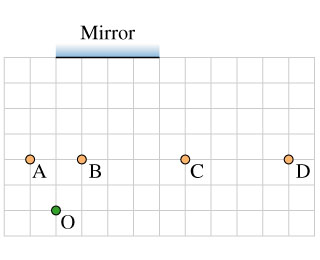
\includegraphics[width=5in]{e1_p1}
\end{figure}

\ep% End Problem

\bp{1}
Two metal balls are the same size but one weighs twice as much as the other. The balls are dropped from the roof of a single-story building at the same instant of time. the time it takes the balls to reach the ground below will be:\\
\begin{choices}
\choice about half as long for the heavier ball as for the lighter one.
\choice about half as long for the lighter ball as for the heavier one.
\choice about the same for both balls.
\choice considerably less for the heavier ball, but not necessarily half as long.
\choice considerably less for the lighter ball, but not necessarily half as long.
\end{choices}
\vfill{}
\ep

\bp{1}
A stone dropped from the roof of a single story building to the surface of the earth:\\
\begin{choices}
\choice reaches a maximum speed quite soon after release and then falls at a constant speed thereafter.
\choice speeds up as it falls because the gravitational attraction gets considerable stronger as the stone gets closer to the earth.
\choice speeds up because of an almost constant force of gravity acting upon it.
\choice falls because of the natural tendency of all objects to rest on the surface of the earth.
\choice falls because of the combined effects of the force of gravity pushing it downward and the force of the air pushing it downward.
\end{choices}
\vfill{}
\ep

\bp{1}
A large truck collides head-on with a small compact car. During the collision:\\
\begin{choices}
\choice the truck exerts a greater amount of force on the car than the car exerts on the truck.
\choice the car exerts a greater amount of force on the truck than the truck exerts on the car.
\choice neither exerts a force on the other, the gets smashed simply because it gets in the way of the truck.
\choice the truck exerts a force on the car but the car does not exert a force on the truck.
\choice the truck exerts the same amount of force on the car as the car exerts on the truck.
\end{choices}
\vfill{}
\ep

\bp{1}
A boy throws a steel ball straight up. Consider the motion of the ball only after it has left the boy's hand but before it touches the ground, and assume that forces exerted by the air are negligible. For these conditions, the force(s) acting on the ball is (are):\\
\begin{choices}
\choice a downward force of gravity along with a steadily decreasing upward force.
\choice a steadily decreasing upward force from the moment it leaves the boy's hand until it reaches its highest point; on the way down there is a steadily increasing downward force of gravity as the object gets closer to earth.
\choice an almost constant downbward force of gravity along with an upward force that steadily decreases until the ball reaches its highest point; on the way down there is only a constant downward force of gravity.
\choice an almost constant force of gravity only.
\choice none of the above. The ball falls back to the ground because of its nautral tendency to rest on the surface of the earth.
\end{choices}
\vfill{}
\ep

\bp{1}
A large truck breaks down on the road and receives a push back into town by a small compact car.\\
While the car, still pushing the truck, is speeding up to get up to the cruising speed:\\
\begin{choices}
\choice the amount of force with which the car pushes on the truck is equal to that with which the truck pushes back on the car.
\choice the amount of force with which the car pushes on the truck is smaller than that with which the truck pushes back on the car.
\choice the amount of force with which the car pushes on the truck is greater than that with which the truck pushes back on the car.
\choice the car's engine is running so the car pushes against the truck, but the truck's engine is not running so the truck cannot push back against the car. The truck is pushed forward simply because it is in the way of the car.
\choice neither the car nor the truck exert any force on the other. The truck is pushed forward simply because it is in the way of the car.
\end{choices}
\vfill{}
\ep

\bp{1}
Consider the situation in the previous problem. After the car reaches the constant cruising speed at which its driver wishes to push the truck:\\
\begin{choices}
\choice the amount of force with which the car pushes on the truck is equal to that with which the truck pushes back on the car.
\choice the amount of force with which the car pushes on the truck is smaller than that with which the truck pushes back on the car.
\choice the amount of force with which the car pushes on the truck is greater than that with which the truck pushes back on the car.
\choice the car's engine is running so the car pushes against the truck, but the truck's engine is not running so the truck cannot push back against the car. The truck is pushed forward simply because it is in the way of the car.
\choice neither the car nor the truck exert any force on the other. The truck is pushed forward simply because it is in the way of the car.
\end{choices}
\vfill{}
\ep

\bp{1}
An elevator is being lifted up an elevator shaft at a constant speed by a steel cable. All frictional forces are negligible. In this situation, forces on the elevator are such that:\\
\begin{choices}
\choice the upward force by the cable is greater than the downward force of gravity.
\choice the upward force by the cable is equal to the downward force of gravity.
\choice the upward force by the cable is smaller than the downward force of gravity.
\choice the upward force by the cable is greater than the sum of the downward force of gravity and a downward force due to the air.
\choice none of the above. (The elevator goes because the cable is being shortened, not because an upward force is exerted on the elevator by the cable).
\end{choices}
\vfill{}
\ep

\bp{1}
A woman exerts a constant horizontal force on a large box. As a result, the box moves across a horizontal force at a constant speed ``$v_0$''.\\
The constant horizontal force applied by the woman:\\
\begin{choices}
\choice has the same magnitude as the weight of the box.
\choice is greater than the weight of the box.
\choice has the same magnitude as the total force which resists the motion of the box.
\choice is greater than the total force which resists the motion of the box.
\choice is greater than either the weight of the box or the total force which resists its motion.
\end{choices}
\vfill{}
\ep

\bp{1}
If the woman in the previous question doubles the constant horizontal force that she exerts on the box to push it on the same horizontal, the box then moves\\
\begin{choices}
\choice with a constant speed that is double the speed ``$v_0$'' in the previous question.
\choice with a constant speed that is greater than the speed ``$v_0$'' in the previous question but not necessarily twice as great.
\choice for a while with a speed that is constant and greater than the speed ``$v_0$'' in the previous question, then with a speed that increases thereafter.
\choice for a while with an increasing speed, then with a constant speed thereafter.
\choice with a continuously increasing speed.
\end{choices}
\vfill{}
\ep

\bp{1}
If the woman in the questions above suddenly stops applying a horizontal force to the block, then the block will:\\
\begin{choices}
\choice immediately come to a stop.
\choice continue moving at a constant speed for a while and then slow to a stop.
\choice immediately start slowing to a stop.
\choice continue at a constant speed.
\choice increasing its speed for a while and then start slowing to a stop.
\end{choices}
\vfill{}
\ep

\bp{1}
The first scientist to introduce the concept of inertia was:\\
\begin{choices}
\choice Galileo.
\choice Copernicus.
\choice Newton.
\choice Aristotle.
\choice Einstein.
\end{choices}
\vfill{}
\ep

\bp{1}
When no forces act on moving objects their paths are normally:\\
\begin{choices}
\choice circles.
\choice straight lines.
\choice ellipses.
\choice all of the above.
\end{choices}
\vfill{}
\ep

\bp{1}
When you quickly jerk a cart forward that has a ball resting in the middle, the\\
\begin{choices}
\choice back of the cart hits the ball.
\choice front of the cart hits the ball.
\choice neither, for the ball rides along in the middle as the cart moves forward.
\end{choices}
\vfill{}
\ep

\bp{1}
Force is a vector quantity because it has both:\\
\begin{choices}
\choice speed and direction.
\choice mass and velocity.
\choice action and reaction counterparts.
\choice magnitude and direction.
\end{choices}
\vfill{}
\ep

\bp{1}
A pair of $\unit[10]{N}$ vectors at right angles has a resultant of about:\\
\begin{choices}
\choice $\unit[20]{N}$.
\choice $\unit[10]{N}$.
\choice $\unit[14]{N}$.
\choice None of the above.
\end{choices}
\vfill{}
\ep

\bp{1}
The net force on any object in equilibrium is:\\
\begin{choices}
\choice equal to its weight.
\choice zero.
\choice less than its weight.
\choice non-zero when motion is involved.
\end{choices}
\vfill{}
\ep

\bp{1}
A hockey puck sliding at constant velocity across the ice is:\\
\begin{choices}
\choice nearly in equilibrium.
\choice in equilibrium.
\choice is nowhere near being in equilibrium.
\choice none of the above.
\end{choices}
\vfill{}
\ep

\bp{1}
\\
\begin{choices}
\choice 
\choice 
\choice 
\choice 
\choice 
\end{choices}
\vfill{}
\ep

\newpage

\end{document}
